\ifx\wholebook\relax \else
\documentclass[b5paper]{article}
\usepackage[nomarginpar
  %, margin=.5in
]{geometry}

\addtolength{\oddsidemargin}{-0.05in}
\addtolength{\evensidemargin}{-0.05in}
\addtolength{\textwidth}{0.1in}
\usepackage[en]{../../../prelude}

\setcounter{page}{1}

\begin{document}

\title{Queue}

\author{Xinyu~LIU
\thanks{{\bfseries Xinyu LIU} \newline
  Email: liuxinyu95@gmail.com \newline}
  }

\maketitle
\fi

\markboth{Queue}{Elementary Algorithms}

\ifx\wholebook\relax
\chapter{Queue}
\numberwithin{Exercise}{chapter}
\fi

\section{Introduction}
\label{introduction}

Queue supports first-in, first-out (FIFO). There are many ways to implement queue, e.g., through linked list, doubly liked list, circular buffer, etc. Okasaki gave 16 different implementations in \cite{okasaki-book}. A queue satisfies the following two requirements:

\begin{enumerate}
\item Add a new element to the tail in constant time;
\item Access or remove an element from head in constant time.
\end{enumerate}

It's easy to realize queue with doubly linked list. We skip this implementation, and focus on using other basic data structures, like (singly) linked list or array.

\section{Linked-list queue}
\index{Queue!linked-list}

We can insert or remove element from the head of a linked list. However, to support FIFO, we have to do one operation in head, and the other in tail. We need $O(n)$ time traverse to reach the tail, where $n$ is the length. To achieve the constant time performance goal, we use an extra variable to record the tail position, and apply a sentinel node $S$ to simplify the empty queue case handling, as shown in figure \cref{fig:empty-list}.

\lstset{frame = single}
\begin{lstlisting}[language = Bourbaki]
data Node<K> {
  Key key
  Node next
}

data Queue {
  Node head, tail
}
\end{lstlisting}

\begin{figure}[htbp]
  \centering
  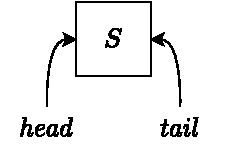
\includegraphics[scale=0.6]{img/empty-list}
  \caption{Both head and tail point to $S$ for empty queue.}
  \label{fig:empty-list}
\end{figure}

The two important queue operations are `enqueue' (also called push, snoc, append, or push back) and `dequeue' (also called pop, or pop front). When implement queue with list, we push on head, and pop from tail.

\begin{algorithmic}[1]
\Function{Enqueue}{$Q, x$}
  \State $p \gets $ \Call{Node}{$x$}
  \State \Call{Next}{$p$} $\gets$ NIL
  \State \textproc{Next}(\Call{Tail}{$Q$}) $\gets p$
  \State \Call{Tail}{$Q$} $\gets p$
\EndFunction
\end{algorithmic}

As there is at least a $S$ node even for empty queue, we need not check if the tail is NIL.

\begin{algorithmic}[1]
\Function{Dequeue}{$Q$}
  \State $x \gets $ \Call{Head}{$Q$}
  \State \textproc{Next}(\Call{Head}{$Q$}) $\gets$ \Call{Next}{$x$}
  \If{$x = $ \Call{Tail}{$Q$}} \Comment{$Q$ is empty}
    \State \Call{Tail}{$Q$} $\gets$ \Call{Head}{$Q$}
  \EndIf
  \State \Return \Call{Key}{$x$}
\EndFunction
\end{algorithmic}

As the $S$ node is ahead of all other nodes, \textproc{Head} actually returns the next node to $S$, as shown in figure \cref{fig:list-queue}. It's easy to expand this implementation to concurrent environment with two locks on the head and tail respectively. $S$ node helps to prevent dead-lock when the queue is empty\cite{PODC96}\cite{SutterDDJ}.

\begin{figure}[htbp]
  \centering
  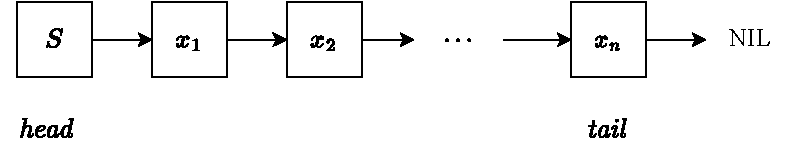
\includegraphics[scale=0.8]{img/slistq}
  \caption{List with $S$ node.}
  \label{fig:list-queue}
\end{figure}

\section{Circular buffer}
\index{Queue!Circular buffer}

Symmetrically, we can append element to the tail of array, but it takes linear time $O(n)$ to remove element from head. This is because we need shift all elements one cell ahead. The idea of circular buffer is to reuse the free cells before the first valid element after we remove elements from head, as shown figure \cref{fig:circular-buffer-queue}, and \cref{fig:circular-buffer}. We can use the head index, the length count, and the size of the array to define a queue. It's empty when the count is 0, it's full when count = size, we can also simplify the enqueue/dequeue implementation with modular operation.

\begin{figure}[htbp]
 \centering
 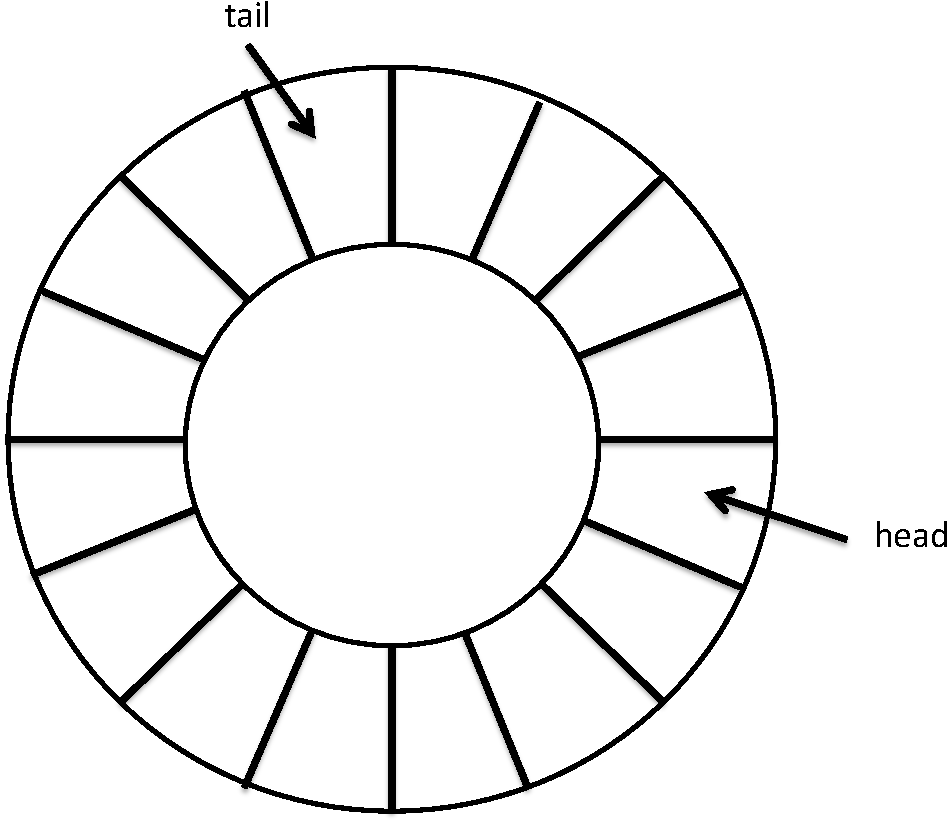
\includegraphics[scale=0.3]{img/ring-buffer}
 \caption{Circular buffer.}
 \label{fig:circular-buffer}
\end{figure}

\begin{figure}[htbp]
 \centering
 \subcaptionbox{Enqueue some elements.}{
 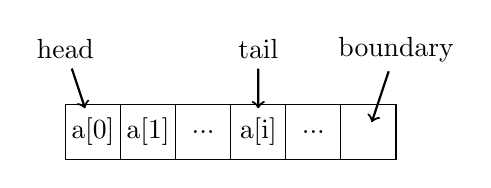
\begin{tikzpicture}[scale=0.7]
    \draw (0, 0) rectangle (1, 1) node (a0) [pos=.5] {a[0]}
          (1, 0) rectangle (2, 1) node [pos=.5] {a[1]}
          (2, 0) rectangle (3, 1) node [pos=.5] {...}
          (3, 0) rectangle (4, 1) node [pos=.5] (ai) {a[i]}
          (4, 0) rectangle (5, 1) node [pos=.5] {...}
          (5, 0) rectangle (6, 1) node (an) [pos=.5] {};
    \draw (0, 2) node (hd) {head}
          (3.5, 2) node (tl) {tail}
          (6, 2) node (bd) {boundary};
    \draw[thick, ->] (hd) edge (a0)
                 (tl) edge (ai)
                 (bd) edge (an);
  \end{tikzpicture}}
 \subcaptionbox{Free cells after dequeue.}{
  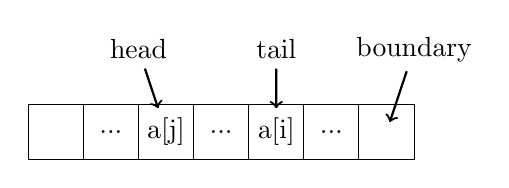
\begin{tikzpicture}[scale=0.7]
    \draw (0, 0) rectangle (1, 1)
          (1, 0) rectangle (2, 1) node [pos=.5] {...}
          (2, 0) rectangle (3, 1) node (aj) [pos=.5] {a[j]}
          (3, 0) rectangle (4, 1) node [pos=.5] {...}
          (4, 0) rectangle (5, 1) node (ai) [pos=.5] {a[i]}
          (5, 0) rectangle (6, 1) node [pos=.5] {...}
          (6, 0) rectangle (7, 1) node (an) [pos=.5] {};
    \draw (2, 2) node (hd) {head}
          (4.5, 2) node (tl) {tail}
          (7, 2) node (bd) {boundary};
    \draw[thick, ->] (hd) edge (aj)
                 (tl) edge (ai)
                 (bd) edge (an);
  \end{tikzpicture}} \\
 \subcaptionbox{Enqueue more elements to the boundary}{
   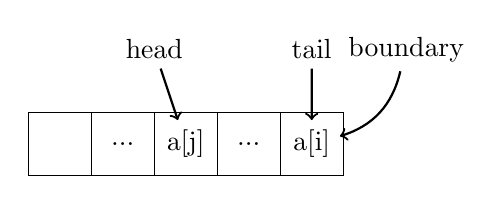
\begin{tikzpicture}[scale=0.8]
    \draw (0, 0) rectangle (1, 1)
          (1, 0) rectangle (2, 1) node [pos=.5] {...}
          (2, 0) rectangle (3, 1) node (aj) [pos=.5] {a[j]}
          (3, 0) rectangle (4, 1) node [pos=.5] {...}
          (4, 0) rectangle (5, 1) node (ai) [pos=.5] {a[i]};
    \draw (2, 2) node (hd) {head}
          (4.5, 2) node (tl) {tail}
          (6, 2) node (bd) {boundary};
    \draw[thick, ->] (hd) edge (aj)
                 (tl) edge (ai)
                 (bd) edge [bend left] (ai);
  \end{tikzpicture}}
 \subcaptionbox{Enqueue the next element to the first cell.}{
    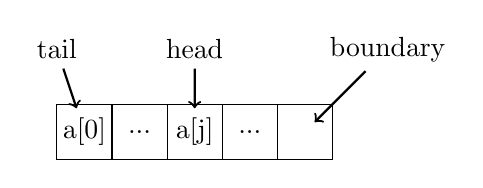
\begin{tikzpicture}[scale=0.7]
    \draw (0, 0) rectangle (1, 1) node (a0) [pos=.5] {a[0]}
          (1, 0) rectangle (2, 1) node [pos=.5] {...}
          (2, 0) rectangle (3, 1) node (aj) [pos=.5] {a[j]}
          (3, 0) rectangle (4, 1) node [pos=.5] {...}
          (4, 0) rectangle (5, 1) node (an) [pos=.5] {};
    \draw (2.5, 2) node (hd) {head}
          (0, 2) node (tl) {tail}
          (6, 2) node (bd) {boundary};
    \draw[thick, ->] (hd) edge (aj)
                 (tl) edge (a0)
                 (bd) edge (an);
  \end{tikzpicture}} \\
 \subcaptionbox{All cells are occupied, full.}{
   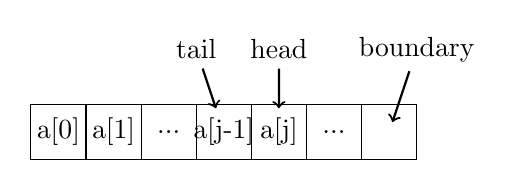
\begin{tikzpicture}[scale=0.7]
    \draw (0, 0) rectangle (1, 1) node [pos=.5] {a[0]}
          (1, 0) rectangle (2, 1) node [pos=.5] {a[1]}
          (2, 0) rectangle (3, 1) node [pos=.5] {...}
          (3, 0) rectangle (4, 1) node (a1j) [pos=.5] {a[j-1]}
          (4, 0) rectangle (5, 1) node (aj) [pos=.5] {a[j]}
          (5, 0) rectangle (6, 1) node [pos=.5] {...}
          (6, 0) rectangle (7, 1) node (an) [pos=.5] {};
    \draw (4.5, 2) node (hd) {head}
          (3, 2) node (tl) {tail}
          (7, 2) node (bd) {boundary};
    \draw[thick, ->] (hd) edge (aj)
                 (tl) edge (a1j)
                 (bd) edge (an);
  \end{tikzpicture}}
 \caption{Circular buffer queue}
 \label{fig:circular-buffer-queue}
\end{figure}

\begin{algorithmic}[1]
\Function{Enqueue}{$Q, x$}
  \If{not \Call{Full}{$Q$}}
    \State \Call{Count}{$Q$} $\gets$ \Call{Count}{$Q$} + 1
    \State tail $\gets $ (\Call{Head}{$Q$} + \Call{Count}{$Q$}) $\bmod$ \Call{Size}{$Q$}
    \State \Call{Buf}{$Q$}[tail] $\gets x$
  \EndIf
\EndFunction
\end{algorithmic}

\begin{algorithmic}[1]
\Function{Dequeue}{$Q$}
  \State $x \gets$ NIL
  \If{not \Call{Empty}{$Q$}}
    \State $h \gets$ \Call{Head}{$Q$}
    \State $x \gets$ \Call{Buf}{$Q$}[$h$]
    \State \Call{Head}{$Q$} $\gets $ (h + 1) $\bmod$ \Call{Size}{$Q$}
    \State \Call{Count}{$Q$} $\gets$ \Call{Count}{$Q$} - 1
  \EndIf
  \State \Return $x$
\EndFunction
\end{algorithmic}

\begin{Exercise}
The circular buffer is allocated with a predefined size. We can use two references head and tail instead of count. How to determine if a circular buffer queue is full or empty? (the head can be either ahead of tail or behind it.)
\end{Exercise}

\section{Paired-list queue}
\index{Queue!Paired-list queue}

We can access list head in constant time, but need linear time to access the tail. We can connect two lists `tail to tail' to implement queue, as shown in figure \cref{fig:horseshoe-magnet}. We define such queue as $(f, r)$, where $f$ is the front list, and $r$ is the rear list. The empty list is $([\ ], [\ ])$. We push new element to the head of $r$, and pop from the tail of $f$. Both are constant time.

\begin{figure}[htbp]
  \centering
  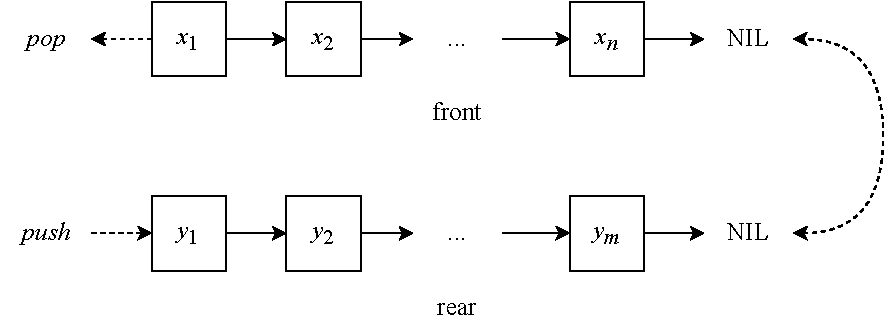
\includegraphics[scale=0.6]{img/paired-listq}
  \caption{paired-list queue.}
  \label{fig:horseshoe-magnet}
\end{figure}

\be
\begin{cases}
push\ x\ (f, r) & = (f, x \cons r) \\
pop\ (x \cons f, r)   & = (f, r) \\
\end{cases}
\ee

$f$ may become empty after a series of pops, while $r$ still contains elements. To continue pop, we reverse $r$ to replace $f$, i.e., $([\ ], r) \mapsto (reverse\ r, [\ ])$. We need check and adjust balance after every push/pop:

\be
\begin{array}{rcl}
\textit{balance}\ [\ ]\ r & = & (\textit{reverse}\ r, [\ ]) \\
\textit{balance}\ f\ r & = & (f, r) \\
\end{array}
\ee

Although the time is bound to linear time when reverse $r$, the amortised performance is constant time. We adjust the push/pop as below:

\be
\begin{cases}
push\ x\ (f, r) & = \textit{balance}\ f\ (x \cons r) \\
pop\ (x \cons f, r)   & = \textit{balance}\ f\ r \\
\end{cases}
\ee

\index{Queue!Paired-array queue}

There is a symmetric implementation with a pair of arrays. Table \cref{tab:array-list-comp} shows the symmetric between list and array. We connect two arrays head to head to form a queue, as shown in figure \cref{fig:horseshoe-array}. When array $R$ becomes empty, we reverse array $F$ to replace $R$.

\begin{table}[htbp]
\centering
\begin{tabular}{l | c | r}
  \hline
  operation & array & list \\
  \hline
  insert to head & $O(n)$ & $O(1)$ \\
  append to tail & $O(1)$ & $O(n)$ \\
  remove from head & $O(n)$ & $O(1)$ \\
  remove from tail & $O(1)$ & $O(n)$ \\
  \hline
\end{tabular}
\caption{array and list}
\label{tab:array-list-comp}
\end{table}

\begin{figure}[htbp]
  \centering
  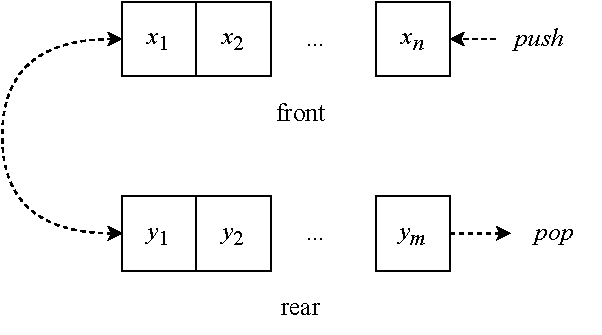
\includegraphics[scale=0.6]{img/paired-arrayq}
  \caption{paired-array queue.}
  \label{fig:horseshoe-array}
\end{figure}

\begin{Exercise}
\Question{Why need balance check and adjustment after push?}
\Question{Prove the amortized performance of paired-list queue is constant time.}
\Question{Implement the paired-array queue.}
\end{Exercise}

\begin{Answer}
\Question{Why need balance check and adjustment after push?

Consider the case, first $push\ a\ ([\ ], [\ ])$, then $pop$.
}
\Question{Prove the amortized performance of paired-list queue is constant time.}
\Question{Implement the paired-array queue.

\begin{algorithmic}[1]
\Function{Push}{$Q, x$}
  \State \textproc{Append}(\Call{Front}{$Q$}, $x$)
\EndFunction
\Statex
\Function{Pop}{$Q$}
  \If{\Call{Rear}{$Q$} $= [\ ]$}
    \State \Call{Rear}{$Q$} $\gets$ \textproc{Reverse}(\Call{Front}{$Q$})
    \State \Call{Front}{$Q$} $\gets [\ ]$
  \EndIf
  \State $n \gets$ \textproc{Length}(\Call{Rear}{$Q$})
  \State $x \gets$ \Call{Rear}{$Q$}[n]
  \State \textproc{Length}(\Call{Rear}{$Q$}) $\gets n - 1$
  \State \Return $x$
\EndFunction
\end{algorithmic}
}
\end{Answer}

\section{Balance Queue}
\index{Queue!Balance Queue}

Although paired-list queue performs in amortized constant time, it is linear time in worse case. For e.g., there is an element in $f$, then repeat pushing $n$ elements. Now it takes $O(n)$ time to pop. The lengths of $f$ and $r$ are unbalance in this case. To solve it, we add another rule: keep the length of $r$ is not greater than $f$, otherwise we reverse.

\be
  |r| \leq |f|
\label{eq:balance-invariant}
\ee

We check the lengths in every push/pop, however, it takes linear time to compute length. We can record the length in a variable, and update it during push/pop. Denote the paired-list queue as $(f, n, r, m)$, where $n = |f|$, $m = |r|$. From the balance rule (\cref{eq:balance-invariant}), we can check the length of $f$ to test if a queue is empty:

\be
  Q = \phi \iff n = 0
\ee

The definition of push/pop change to:

\be
\begin{cases}
  push\ x\ (f, n, r, m) & = \textit{balance}\ (f, n,  x \cons r, m + 1) \\
  pop\ (x \cons f, n, r, m) & = \textit{balance}\ (f, n - 1, r, m) \\
\end{cases}
\ee

Where \textit{balance} is defined as:

\be
\textit{balance}\ (f, n, r, m) = \begin{cases}
  m \leq n: & (f, n, r, m) \\
  \text{otherwise}: & (f \doubleplus reverse\ r, m + n, [\ ], 0)\\
\end{cases}
\ee

\section{Real-time queue}
\index{Queue!Real-time queue}

It still takes linear time to reverse, concatenate lists in balanced queue. A real-time queue need guarantee constant time in every push/pop operation. The performance bottleneck happens in $f \doubleplus reverse\ r$. At this time, $m > $, breaks the balance rule. Since $m, n$ are integers, we know $m = n + 1$. $\doubleplus$ takes $O(n)$ time, and reverse takes $O(m)$ time. The total time is bound to $O(n + m)$, which is proportion to the number of elements. Our solution is to distribute this computation to multiple push and pop operations. Let's revisit the tail recursive\cite{wiki-tail-call}\cite{recursion} reverse:

\be
reverse\ = reverse'\ [\ ]
\ee

This is in Curried form, where:

\be
\begin{array}{rcl}
\textit{reverse}'\ a\ [\ ] & = & a \\
\textit{reverse}'\ a\ (x \cons xs) & = & \textit{reverse}'\ (x \cons a)\ xs \\
\end{array}
\ee

We can turn the tail recursive implementation to stepped computation. We model it as a series of state transformation. Define a state machine with two states: reverse state $S_r$, and complete state $S_f$. We {\em slow-down} the reverse computation as below:

\be
\begin{array}{rcl}
step\ S_r\ a\ [\ ] & = & (S_f, a) \\
step\ S_r\ a\ (x \cons xs) & = & (S_r, (x \cons a), xs) \\
\end{array}
\ee

Each step, we check and transform the state. $S_r$ means the reverse is on going. If there is no remaining element to reverse, we change the state to $S_f$ (done); otherwise, we pick the head element $x$, link it ahead of $a$. This step terminates, but not continues to recursion. The new state with the intermediate reverse result will be input to the next $step$. For example:

\[
\begin{array}{rcl}
step\ S_r\ \text{``hello''}\ [\ ] & = & (S_r, \text{``ello''}, \text{``h''}) \\
step\ S_r\ \text{``ello''}\ \text{``h''} & = & (S_r, \text{``llo''}, \text{``eh''}) \\
... & & \\
step\ S_r\ \text{``o''}\ \text{``lleh''} & = & (S_r, [\ ], \text{``olleh''}) \\
step\ S_r\ [\ ]\ \text{``olleh''} & = & (S_f, \text{``olleh''})
\end{array}
\]

We can next distribute the reverse steps to push/pop operations. However, it only solves half problem. We next need slow-down $\doubleplus$ computation, which is more complex. We use state machine too. To concatenate $xs \doubleplus ys$, we first reverse $xs$ to $\overleftarrow{xs}$, then pick elements form $\overleftarrow{xs}$ one by one, and link each head of $ys$. The idea is similar to $\textit{reverse}'$:

\be
  \begin{array}{rcl}
    xs \doubleplus ys & = & (reverse\ reverse\ xs) \doubleplus ys \\
             & = & (reverse'\ [\ ]\ (reverse\ xs)) \doubleplus ys \\
             & = & reverse'\ ys\ (reverse\ xs) \\
             & = & reverse'\ ys\ \overleftarrow{xs}
  \end{array}
\ee

We need add another state. After reverse $r$, we step by step concatenate from $\overleftarrow{f}$. The three states are: $S_r$ of reverse, $S_c$ of concatenate, $S_f$ of completion. The two phases are:

\begin{enumerate}
\item Reverse $f$ and $r$ in parallel to: $\overleftarrow{f}$ and
$\overleftarrow{r}$ step by step;
\item Stepped taking elements from $\overleftarrow{f}$, and link each ahead of $\overleftarrow{r}$.
\end{enumerate}

\be
\begin{array}{rcll}
next\ (S_r, f', x \cons f, r', y \cons r) & = & (S_r, x \cons f', f, y \cons r', r) & \text{reverse}\ f, r\\
next\ (S_r, f', [\ ], r', [y]) & = & next\ (S_c, f', y \cons r') & \text{reverse done, start concatenation}\\
next\ (S_c, a, [\ ]) & = & (S_f, a) & \text{done}\\
next\ (S_c, a, x \cons f') & = & (S_c, x \cons a, f') & \text{concatenation}\\
\end{array}
\ee

We need arrange these steps to each push/pop next. From the balance rule, when $m = n + 1$, we kick off $f \doubleplus reverse\ r$. it takes $n + 1$ steps to reverse $r$, within these steps, we reverse $f$ in parallel. After that, we use another $n + 1$ steps to concatenate. $2n + 2$ steps in total. The critical question is: Before we complete the $2n + 2$ steps, will the queue become unbalanced due to a series of push/pop operations?

Luckily, repeat pushing won't break the balance rule again before we complete $f \doubleplus reverse\ r$ in $2n + 2$ steps. We will obtain a new front list $f' = f \doubleplus reverse\ r$ after $2n + 2$ steps, while the time to break the balance rule again is:

\be
  \begin{array}{rcl}
  |r'| & = & |f'| + 1 \\
       & = & |f| + |r| + 1 \\
       & = & 2n + 2
  \end{array}
\ee

Thanks to the balance rule. It means even repeat pushing as many elements as possible, from the previous to the next time when the queue is unbalanced, the $2n + 2$ steps are guaranteed to be completed, hence the new $f$ is ready. We can next safely start to compute $f' \doubleplus reverse\ r'$.

However, pop may happen before the completion of $2n + 2$ steps. We are facing the situation that needs extract element from $f$, while the new front list $f' = f \doubleplus reverse\ r$ hasn't been ready yet. To solve this issue, we duplicate a copy of $f$ when doing $reverse\ f$. We are save even repeat pop for $n$ times. Table \cref{tab:pop-before-n} shows the queue during phase 1 (reverse $f$ and $r$ in parallel)\footnote{Although it takes linear time to duplicate a list, however, the one time copying won't happen at all. We actually duplicate the reference to the front list, and delay the element level copying to each step}.

\begin{table}[htbp]
\centering
\begin{tabular}{c | c | c}
  $f$ copy & on-going part & new $r$ \\
  \hline
  $\{ f_i, f_{i+1}, ..., f_n \}$ & $(S_r, \tilde{f}, ..., \tilde{r}, ...)$ & $ \{ ... \}$ \\
  first $i-1$ elements out & intermediate $\overleftarrow{f}$, $\overleftarrow{r}$ & newly pushed
\end{tabular}
\caption{Before completion of the first $n$ steps.}
\label{tab:pop-before-n}
\end{table}

The copy of $f$ is exhausted after repeated $n$ pops. We are about to stepped concatenation. What if pop happens at this time? Since $f$ is exhausted, it becomes $[\ ]$. We needn't concatenate anymore. This is because $f \doubleplus \overleftarrow{r} = [\ ] \doubleplus \overleftarrow{r} = \overleftarrow{r}$. In fact, we only need to concatenate the elements in $f$ that haven't been popped. Because we pop elements from the head of $f$, we use a counter to record the remaining elements in $f$. It's initialized as 0. We apply +1 every time when reverse an element in $f$. It means we need concatenate this element in the future; Whenever pop happens, we apply -1, means we needn't concatenate this one any more. We also decrease it during concatenation process, and cancel the process when it is 0. Below is the updated state transformation:

\be
\begin{array}{rcll}
next\ (S_r, n, f', x \cons f, r', y \cons r) & = & (S_r, n + 1, x \cons f', f, y \cons r', r) & \text{reverse}\ f, r\\
next\ (S_r, n, f', [\ ], r', [y]) & = & next\ (S_c, n, f', y \cons r') & \text{reverse done, start concatenation}\\
next\ (S_c, 0, a, f) & = & (S_f, a) & \text{done}\\
next\ (S_c, n, a, x \cons f') & = & (S_c, n - 1, x \cons a, f') & \text{concatenation}\\
next\ S_0 & = & S_0 & \text{idle} \\
\end{array}
\ee

We define addition idle state $S_0$ to simplify the transition logic. The queue contains 3 parts: the front list $f$ with its length $n$, the state $S$ of on going $f \doubleplus reverse\ r$, and the rear list $r$ with its length $m$. Denoted as $(f, n, S, r, m)$. The empty queue is $([\ ], 0, S_0, [\ ], 0)$. We can tell a queue is empty when $n = 0$ according to the balance rule. The push/pop are updated as:

\be
\begin{cases}
  push\ x\ (f, n, S, r, m) & = balance\ f\ n\ S\ (x \cons r)\ (m + 1) \\
  pop\ (x \cons f, n, S, r, m) & = balance\ f\ (n - 1)\ (abort\ S)\ r\ m \\
\end{cases}
\ee

Where $abort$ decrease the counter in pop to cancel an element for concatenation. We'll define it later. $balance$ triggers stepped $f \doubleplus reverse\ r$ if the queue is unbalanced, else runs a step:

\be
balance\ f\ n\ S\ r\ m = \begin{cases}
  m \leq n: & step\ f\ n\ S\ r\ m \\
  \text{otherwise}: & step\ f\ (n + m)\ (next\ (S_r, 0, [\ ], f, [\ ], r))\ [\ ]\ 0 \\
\end{cases}
\ee

Where $step$ transforms the state machine to next state. It ends with the idle state $S_0$ when completes.

\be
step\ f\ n\ S\ r\ m = queue\ (next\ S)
\ee

Where:

\be
\begin{array}{rcll}
queue\ (S_f, f') & = & (f', n, S_0, r, m) & \text{replace $f$ with $f'$} \\
queue\ S' & = & (f, n, S', r, m) & \\
\end{array}
\ee

We define $abort$ to cancel an element:

\be
\begin{array}{rcl}
abort\ (S_c, 0, (x \cons a), f') & = & (S_f, a) \\
abort\ (S_c, n, a, f') & = & (S_c, n - 1, a, f') \\
abort\ (S_r, n, f' f, r' r) & = & (S_r, n - 1, f', f, r', r) \\
abort\ S & = & S
\end{array}
\ee

\begin{Exercise}
\Question{Why need rollback an element (we cancelled the previous `cons', removed $x$ and return $a$ as the result) when $n=0$ in $abort$? }
\end{Exercise}

\section{Lazy real-time queue}
\index{Queue!Lazy real-time queue}

The key to realize real-time queue is to break down the expensive
$f \doubleplus reverse\ r$. We can simplify it with lazy evaluation. Assume function $rotate$ compute $f \doubleplus reverse\ r$ in steps, i.e., below two functions are equivalent with an accumulator $a$.
\be
  rotate\ xs\ ys\ a = xs \doubleplus (reverse\ ys) \doubleplus a
  \label{eq:rot-def}
\ee

We initialize $xs$ as the front list $f$, $ys$ as the rear list $r$,
the accumulator $a$ empty $[\ ]$. We implement $rotate$ from the edge case:

\be
  rotate\ [\ ]\ [y]\ a = y \cons a
\ee

The recursive case is:

\be
  \begin{array}{cll}
  & rotate\ (x \cons xs)\ (y \cons ys)\ a & \\
  = & (x \cons xs) \doubleplus (reverse\ (y \cons ys)) \doubleplus a & \text{from (\cref{eq:rot-def})} \\
  = & x : (xs \doubleplus reverse\ (y \cons ys)) \doubleplus a) & \text{concatenation is associative} \\
  = &  x : (xs \doubleplus reverse\ ys \doubleplus (y \cons a)) & \text{reverse property, and associative} \\
  = & x : rotate\ xs\ ys\ (y \cons a) & \text{reverse of (\cref{eq:rot-def})}
  \end{array}
\ee

Summarize them together:

\be
\begin{array}{rcl}
rotate\ [\ ]\ [y]\ a & = & y \cons a \\
rotate\ (x \cons xs)\ (y \cons ys)\ a & = & x : rotate\ xs\ ys\ (y \cons a) \\
\end{array}
\ee

In lazy evaluation settings, (:) is delayed to push/pop, hence the $rotate$ is broken down. We change the paired-list queue definition to $(f, r, rot)$, where $rot$ is the on going $f \doubleplus reverse\ r$ computation. It is initialized empty $[\ ]$.

\be
\begin{cases}
push\ x\ (f, r, rot) & = balance\ f\ (x \cons r)\ rot \\
pop\ (x \cons f, r, rot) & = balance\ f\ r\ rot \\
\end{cases}
\ee

Every time, $balance$ advances the rotation one step, and starts another round when completes.

\be
\begin{array}{rcll}
balance\ f\ r\ [\ ] & = & (f', [\ ], f') & \text{其中}: f' = rotate\ f\ r\ [\ ] \\
balance\ f\ r\ (x \cons rot) & = & (f, r, rot) & \text{推进轮转}\\
\end{array}
\ee

\begin{Exercise}
Implement bidirectional queue, support add/remove elements on both head and tail in constant time.
\end{Exercise}

\section{Appendix - example programs}

List implemented queue:

\begin{lstlisting}[language = Bourbaki]
Queue<K> enQ(Queue<K> q, K x) {
    var p = Node(x)
    p.next = null
    q.tail.next = p
    q.tail = p
    return q
}

K deQ(Queue<K> q) {
    var p = q.head.next   //the next of S
    q.head.next = p.next
    if q.tail == p then q.tail = q.head //empty
    return p.key
}
\end{lstlisting}

Circular buffer queue:

\begin{lstlisting}[language = Bourbaki]
data Queue<K> {
    [K] buf
    int head, cnt, size

    Queue(int max) {
        buf = Array<K>(max)
        size = max
        head = cnt = 0
    }
}
\end{lstlisting}

Enqueue, dequeue implementation for circular buffer queue:

\begin{lstlisting}
N offset(N i, N size) = if i < size then i else i - size

void enQ(Queue<K> q, K x) {
    if q.cnt < q.size {
        q.buf[offset(q.head + q.cnt, q.size)] = x;
        q.cnt = q.cnt + 1
    }
}

K head(Queue<K> q) = if q.cnt == 0 then null else q.buf[q.head]

K deQ(Queue<K> q) {
    K x = null
    if q.cnt > 0 {
        x = head(q)
        q.head = offset(q->head + 1, q->size);
        q.cnt = q.cnt -1
    }
    return x
}
\end{lstlisting}

Real-time queue:

\begin{Haskell}
data State a = Empty
             | Reverse Int [a] [a] [a] [a] -- n, acc f, f, acc r, r
             | Concat Int [a] [a]          -- n, acc, reversed f
             | Done [a]  -- f' = f ++ reverse r

-- f, n = length f, state, r, m = length r
data RealtimeQueue a = RTQ [a] Int (State a) [a] Int

push x (RTQ f n s r m) = balance f n s (x:r) (m + 1)

pop (RTQ (_:f) n s r m) = balance f (n - 1) (abort s) r m

top (RTQ (x:_) _ _ _ _) = x

balance f n s r m
    | m <= n =  step f n s r m
    | otherwise = step f (m + n) (next (Reverse 0 [] f [] r)) [] 0

step f n s r m = queue (next s) where
  queue (Done f') = RTQ f' n Empty r m
  queue s' = RTQ f n s' r m

next (Reverse n f' (x:f) r' (y:r)) = Reverse (n + 1) (x:f') f (y:r') r
next (Reverse n f' [] r' [y]) = next $ Concat n (y:r') f'
next (Concat 0 acc _) = Done acc
next (Concat n acc (x:f')) = Concat (n-1) (x:acc) f'
next s = s

abort (Concat 0 (_:acc) _) = Done acc -- rollback 1 elem
abort (Concat n acc f') = Concat (n - 1) acc f'
abort (Reverse n f' f r' r) = Reverse (n - 1) f' f r' r
abort s = s
\end{Haskell}

Lazy real-time queue:

\begin{Haskell}
data LazyRTQueue a = LQ [a] [a] [a] -- front, rear, f ++ reverse r

empty = LQ [] [] []

push (LQ f r rot) x = balance f (x:r) rot

pop (LQ (_:f) r rot) = balance f r rot

top (LQ (x:_) _ _) = x

balance f r [] = let f' = rotate f r [] in LQ f' [] f'
balance f r (_:rot) = LQ f r rot

rotate [] [y] acc = y:acc
rotate (x:xs) (y:ys) acc = x : rotate xs ys (y:acc)
\end{Haskell}

\ifx\wholebook\relax \else
\section{Answers}
\shipoutAnswer

\begin{thebibliography}{99}

\bibitem{PODC96}
Maged M. Michael and Michael L. Scott. ``Simple, Fast, and Practical Non-Blocking and Blocking Concurrent Queue Algorithms''. \url{http://www.cs.rochester.edu/research/synchronization/pseudocode/queues.html}

\bibitem{SutterDDJ}
Herb Sutter. ``Writing a Generalized Concurrent Queue''. Dr. Dobb's Oct 29, 2008. \url{http://drdobbs.com/cpp/211601363?pgno=1}

\bibitem{CLRS}
Thomas H. Cormen, Charles E. Leiserson, Ronald L. Rivest and Clifford Stein. ``Introduction to Algorithms, Second Edition''. The MIT Press, 2001. ISBN: 0262032937.

\bibitem{okasaki-book}
Chris Okasaki. ``Purely Functional Data Structures''. Cambridge university press, (July 1, 1999), ISBN-13: 978-0521663502

\bibitem{tail-call}
Wikipedia. ``Tail-call''. \url{https://en.wikipedia.org/wiki/Tail_call}

\bibitem{recursion}
Wikipedia. ``Recursion (computer science)''. \url{https://en.wikipedia.org/wiki/Recursion_(computer_science)#Tail-recursive_functions}

\bibitem{SICP}
Harold Abelson, Gerald Jay Sussman, Julie Sussman. ``Structure and Interpretation of Computer Programs, 2nd Edition''. MIT Press, 1996, ISBN 0-262-51087-1

\end{thebibliography}

\expandafter\enddocument
\fi
